\chapter{第1講：弦理論專題}

\lectureoverview{在\(1+1\)維度中，玻色化、電--磁對偶、D膜、強耦合相變、湧現幾何，以及弦真空的組合景觀，都使還原論面臨的挑戰更加尖銳。同一個物理系統可能有截然不同的基本描述；哪一種描述較簡單，取決於耦合與幾何。}

\section{還原論、複雜性與簡單性問題}

Susskind以一句刻意選得耳熟能詳的哲學口號開場：大的事物由小的事物構成，小的事物又由更小的事物構成。接著，他提出同一想法中更宏大的版本，也是對基礎物理真正重要的版本：愈深入底層，物件不只應該愈小，也應該愈簡單。他用房子和磚塊作比喻：房子由磚塊構成，沒有人會把房子誤認為一塊磚。磚塊比較小，也比較簡單。

本講首先以粒子物理的實際情況檢視這項預期。如果還原論真能在這種強意義下帶來愈來愈簡單的描述，人們或許會預期當代基本粒子物理已相當精簡。然而，Susskind強調，即使還沒把量子引力納入考量，帳目看起來就已經相當凌亂。講座中的數字只是粗略估計，但這種粗略正是論點的一部分：
\begin{equation}
\begin{aligned}
N_{\mathrm{species}}&\sim 75,\\
N_{\mathrm{independent}}&\sim 10\text{--}20,\\
N_{\mathrm{parameters}}&\sim 20.
\end{aligned}
\end{equation}
即便如此，故事仍未結束。標準模型不包含重力，無法解釋暗物質，也沒有提供暴脹所需的額外結構，還面臨嚴重的精細調整問題。加入通常用來修補這些問題的機制，只會使數目增加。講座以超對稱為例。在講座當時，許多物理學家期待大型強子對撞機能找到超伴粒子；Susskind則強調，相應的擴充會增加一百多個參數，並不會立即讓帳目變得簡單。他用下式概略表達這個意思：
\begin{equation}
N_{\mathrm{parameters}}^{\mathrm{extended}} \sim 200.
\end{equation}
這些數字刻意採用粗略估計，也反映了當時的歷史背景。它們要說明的是，更深層的描述在粒子清單與測得常數的層面上，未必看起來更簡單。

這番數量上的抱怨還不是Susskind的主要論點，而只是前奏。真正更深一層、也推動本講其餘內容的主張是：現代量子場論與弦理論並未明確支持一種唯一且不受耦合影響的磚塊與房子之分。接下來的例子要說明，``基本''究竟代表什麼，可能取決於哪些變數最有效率。

\section{玻色化：固定基本性概念的首次動搖}

Susskind的第一個理論例子來自\(1+1\)維量子場論，也就是一維空間加上一維時間。他一開始就說明，自己不會詳細推導這種等價性；重點不在形式上的證明，而在於它帶來的概念啟示。

先從費米子場論出發。費米子場記為\(\psi\)。兩個彼此接近的費米子可以組成玻色複合態，相應的玻色子場記為\(\phi\)。乍看之下，層級關係似乎很清楚：\(\psi\)是基本的，\(\phi\)則是複合或有效變數。在講座中，玻色子正是以這種方式引入：它是一個能產生費米子束縛對的場。

然而，人們發現，同一個理論也可以從相反的起點改寫。可以從玻色子場\(\phi\)出發；在這種描述中，費米子不再是點狀的組成成分，而是以玻色子場的扭結形式出現。這是一種延展構型，其中\(\phi\)在兩個漸近值之間平滑地變化。講座中最基本的數學內容，就是這種漸近結構：
\begin{equation}
\phi(x\to -\infty)=\phi_-,
\qquad
\phi(x\to +\infty)=\phi_+.
\end{equation}
一個方便的示意形式是
\begin{equation}
\phi(x)\approx \frac{\phi_++\phi_-}{2}
+
\frac{\phi_+-\phi_-}{2}\tanh\!\left(\frac{x}{\ell}\right),
\end{equation}
其中\(\ell\)是過渡區域的寬度。

\editorialnote{雙曲正切剖面是講座所畫扭結的一種標準平滑形式，並非講座中推導出的公式。精確的玻色化對照關係取決於模型；概念上的重點，是費米子激發與玻色子場拓撲孤子之間的對換。}

講座中的皮帶類比相當具體，值得保留。平直而未扭轉的皮帶，代表沒有扭結的構型。若將一端旋轉\(2\pi\)，皮帶在遠處仍會回到相同的局部方向，但中間必須經過一段延展的扭轉區域。那段扭轉區域就是扭結。在玻色子描述中，費米子正是由這樣的延展物件表示。

引入耦合後，這個重點就更加清楚。Susskind在此例中將耦合稱為\(G\)。他要說的不是兩種描述彼此略有關聯，而是兩者的效率取決於參數所在的範圍：
\begin{align}
G \ll 1
&\Rightarrow
\ell\text{ small, tight kink; }\psi\text{ efficient},\\
G \gg 1
&\Rightarrow
\ell\text{ large, broad kink; }\phi\text{ efficient}.
\end{align}
當\(G\)很小時，扭結很窄，費米子看起來是簡單的物件。隨著\(G\)增大，扭結變寬，費米子也愈不像點狀物件。此時以玻色子變數描述會更精簡。

\paragraph{示意性的更新規則。}
\begin{enumerate}
\item 從以\(\psi\)描述的費米子理論出發。
\item 找出以\(\phi\)描述的玻色複合態。
\item 將同一個理論完全改寫為以\(\phi\)描述。
\item 在玻色子描述中，費米子會以寬度為\(\ell\)的扭結重新出現。
\item 當\(G\ll 1\)時，\(\ell\)很小，費米子描述最簡單。
\item 當\(G\)較大時，\(\ell\)會增大，玻色子描述便更簡單。
\end{enumerate}

這是第一個明確反例，挑戰了固定不變的``房子與磚塊''圖像。講座的重點不只是複合物件確實存在，更在於何者算是基本變數，會隨耦合而改變。

\section{電荷、磁單極子與弱耦合、強耦合}

Susskind接著問，更熟悉的粒子物理中是否也有類似情況。例子是電荷與磁單極子。在這裡的語言中，普通的帶電粒子，例如電子，就是電單極子：局域的電場源。磁單極子則透過條形磁鐵的類比引入。如果能以某種方式把條形磁鐵的一端分離出來，而不帶上那根看不見的連接棒，它的場線就會和電荷的場線完全相同，只不過是磁場而非電場。

相關的控制參數是精細結構常數\(\alpha\)。在講座中，Susskind以啟發式的方式將它視為電荷的平方：
\begin{equation}
\alpha \sim e^2.
\end{equation}
他也給出一種粗略的操作性解釋：這個常數衡量電子有多容易輻射。他用加速電子在相關意義上會輻射約``\(1/100\)''個光子，來概括輻射強度。以講座中粗略的數值來說：
\begin{equation}
\alpha \approx 10^{-2}.
\end{equation}
這不是要建立精確的定義慣例，而是一種教學上的說法，用來表達電荷很弱。

\editorialnote{弱--強的關係，在Dirac量子化中有精確的先例。在一種常見的慣例下，電荷與磁荷滿足\(e g_m=2\pi n\)。因此，弱電耦合對應強磁耦合，不過精確的數值因子與受保護的質量關係仍取決於理論。}

當\(\alpha\ll 1\)時，電子是簡單的物件。它的電場很弱，真空極化雲也很稀薄，因此看起來幾乎是點狀的。磁單極子則恰好相反：它的場極強，周遭受到劇烈擾動，而且範圍廣、結構複雜又沉重。Susskind以弱--強的方式概括這種情況：
\begin{equation}
\begin{aligned}
\alpha \ll 1
&\Rightarrow \text{simple electron;}\\
&\phantom{\Rightarrow{}}\text{heavy, extended monopole},\\
\alpha \gg 1
&\Rightarrow \text{simple monopole;}\\
&\phantom{\Rightarrow{}}\text{heavy, structured electron}.
\end{aligned}
\end{equation}
講座並未推導磁單極子的質量公式，也不需要這麼做。重點在於定性趨勢。隨著\(\alpha\)增大，電子的場變強，結構也愈來愈大；磁單極子則逐漸縮小、變輕。當耦合遠大於1時，有效的描述便會互換：磁單極子變得簡單，電子則變得複雜。

這正是先前玻色化例子所帶出的場論版教訓。基本與複合之間的區分並非絕對，而是取決於耦合。

\begin{classroomqa}
\audiencequestion{如果還原論並非可靠的指引，為什麼物理學家仍仰賴微積分？微積分似乎會把系統分割成任意小的部分。\lecturetimestamp{00:21:21}}
\lecturerresponse{微積分描述的是連續變化，並不會指出理論中的基本物件。量子場在各種距離尺度上都會漲落，形成無窮無盡的層級，而不是一個最終且平滑的底層，讓人可以一勞永逸地判定何者為基本。}
\end{classroomqa}

對話接著有人提出，這種層級結構就像分形。Susskind接受這個類比，並進一步指出：量子場在所有尺度上都會漲落，因此在經典意義下從來不平滑。這種劇烈變化是量子場論在數學上難以處理的原因之一；運用一般微積分時，必須使用重整化後的量，而不能把微觀場當成樸素而平滑的場。

\section{弦、D膜與弱--強對偶性的再現}

講座接下來的轉折刻意從一個天真的想法出發：如果弦理論是研究基本構成單元的理論，答案想必很簡單——構成單元就是弦。Susskind明白說出這項預期，接著便在講座下一部分逐步拆解它。

\subsection{為什麼弦並非全部}

第一個複雜之處，是D膜無可避免地存在。D\(p\)膜是\(p\)維物件，弦可以終止於其上。字母\(D\)來自Dirichlet邊界條件，但它的作用遠比名稱重要：這些物件是理論的一部分，不能忽略，也不是可有可無的裝飾。

最簡單的例子如下：
\begin{itemize}
\item D0膜，是點狀物件；
\item D1膜，也稱為D弦，是弦狀物件；
\item F弦，也就是普通的基本弦。
\end{itemize}
D0膜是沉重的點狀位置，任意數量的F弦都可以終止於其上。D1膜則是沉重的纜索狀物件，比F弦粗得多，單位長度的質量也大得多，但同樣可以讓F弦終止於其上。在弱耦合下，講座並未把這些物件描述成同樣基本的替代選項。D膜被介紹為沉重、有結構、看似複合的物件，然而理論仍要求它們存在。

\editorialnote{講座這部分討論的奇數維膜理論是IIB型弦理論。其穩定的D膜具有奇數空間維度，包括D1膜和D3膜。Susskind暫時不說明這些名稱，因為當下的主題是對偶性模式，而非分類。}

\paragraph{記號。}
Susskind在講座不同部分使用\(G\)和\(g\)時，記號並不完全一致。本文以\(G\)專指玻色化例子中的耦合，以\(g\)表示弦耦合。

弦耦合\(g\)是以操作方式定義，而非從公理出發定義。它是衡量漲落中的弦分裂並形成子弦之機率的參數。因此，Susskind會直接把它和QED中的\(\alpha\)相比。講座也特別指出，張力就是單位長度的能量：
\begin{equation}
T=\frac{E}{L}=\frac{M}{L}.
\end{equation}

對F弦與D弦而言，標準張力公式明確呈現弱--強耦合之間的比較：
\begin{equation}
T_{\mathrm{F1}}=\frac{1}{2\pi\alpha'},
\qquad
T_{\mathrm{D1}}=\frac{1}{2\pi\alpha' g_s},
\qquad
\frac{T_{\mathrm{D1}}}{T_{\mathrm{F1}}}=\frac{1}{g_s}.
\end{equation}
\editorialnote{這些張力公式採用標準歸一化，呈現講座中纜索與細線之間的定性比較。這些公式是編輯補充的；講座只討論張力隨耦合變化的尺度關係。}

\subsection{F弦與D弦}

弱--強的故事接著以弦的語言重演。在小耦合下，F 弦輕而細，接近人們最初對基本物體的直觀想像。D 弦則粗而重，內含豐富的 F 弦結構。隨著耦合增大，F 弦更容易分裂；子弦雲在它周圍不斷增生，使它變得更重、更複雜。與此同時，D 弦越來越難以放出如今已變得很重的 F 弦，因此周圍的結構逐漸稀薄，它也變得更輕、更像一條線。因此，講座中的弱--強對應關係是
\begin{align}
g \ll 1
&\Rightarrow
\begin{gathered}
\text{F-string light and thin;}\\
\text{D-string heavy and structured},
\end{gathered}\\
g \sim 1
&\Rightarrow
\text{F-string and D-string comparable},\\
g \gg 1
&\Rightarrow
\begin{gathered}
\text{D-string light and thin;}\\
\text{F-string heavy and structured}.
\end{gathered}
\end{align}
Susskind 指出，在 \(g\sim 1\) 附近，兩種描述的差異不再鮮明。超過這個範圍後，兩者實際上會交換角色。這是弦論版的電子--磁單極子互換，公認的名稱是 S 對偶。

弦閉合成環後，也可以看到同樣的角色互換。在弱耦合下，小型F弦環是輕的類粒子激發；相應的D弦環則沉重而複雜。強耦合時兩者角色反轉：D弦環成為較輕的描述，而由此得到的輕閉弦激發中包含引力子。Susskind藉此例指出，即使是熟悉粒子的身分，也可能取決於採用對偶性的哪一側描述。

講座把這個觀點再推進一步。在理想化理論中，耦合不只是可以任意調整的數值；它的表現如同一個場。示意地說：
\begin{equation}
g = g(x).
\end{equation}
因此，空間不同區域可能適合不同的對偶描述：某個區域以F弦為輕的變數，另一個區域則以D弦為輕的變數；兩者之間沒有哪一種描述特別簡單。對Susskind來說，弦理論並未恢復簡單的還原論圖像，反而讓這種模糊性更加徹底。

\editorialnote{在微擾弦理論中，局部耦合由膨脹子決定：\(g_s(x)=e^{\Phi(x)}\)。因此，寫成\(g=g(x)\)並非只是類比，儘管在現實的緊緻化中，通常會產生限制這類變化的勢。}

\begin{classroomqa}
\audiencequestion{如果耦合變化得夠大，使另一個區域中的D弦比F弦更輕，這種變化會影響可觀測的譜嗎？\lecturetimestamp{00:34:15}}
\lecturerresponse{會。這也是為什麼不能直接把這個完全對稱、在數學上可精確掌控的模型，等同於我們的世界。它所揭示的是自洽量子理論可能具有的性質，而不是自然界實際粒子譜的直接描述。}
\end{classroomqa}

\begin{classroomqa}
\audiencequestion{D2膜是否也有類似的對偶描述？\lecturetimestamp{00:34:39}}
\lecturerresponse{有，但不是另一種D弦式的角色互換。偶數維膜的情況會引出膜的詮釋與額外空間維度，這就是接下來要介紹的構造。}
\end{classroomqa}

\begin{classroomqa}
\audiencequestion{弦分裂的機率提高，是否就能解釋內部結構變得更複雜？\lecturetimestamp{00:34:53}}
\lecturerresponse{可以。為了具體說明這個機制，回到QED：電子發射光子，光子漲落成帶電粒子對，而那些帶電的線又會再次輻射。耦合增大時，這個層級結構就不再那麼稀疏。}
\end{classroomqa}

\subsection{以問答為引導，回到量子電動力學}

接著，一名學生問，分裂機率提高，是否就單純代表``上游''的結構變得更複雜。Susskind回到量子電動力學，再次畫出電子的世界線來回答。這段回顧很重要，因為它表明弦的故事並非孤立的特例，而是弱--強耦合模式的另一個例子。

\begin{figure}[htbp]
\centering
\begin{tikzpicture}[scale=1.0]
\draw[->] (-1.2,0) -- (3.7,0) node[right] {space};
\draw[->] (0,-0.2) -- (0,4.3) node[above] {time};

\draw[line width=0.9pt] (0,0.2) -- (0,4.0);
\node[left] at (0,3.55) {\(e^{-}\)};

\draw[line width=0.8pt] (0,1.0) -- (0.18,1.08) -- (0.36,0.92) -- (0.54,1.10) -- (0.72,0.94) -- (0.90,1.12) -- (1.08,0.96) -- (1.26,1.14);
\draw[line width=0.8pt] (0,2.35) -- (-0.18,2.43) -- (-0.36,2.27) -- (-0.54,2.45) -- (-0.72,2.29) -- (-0.90,2.47);

\draw[line width=0.8pt] (1.26,1.14) -- (1.48,1.42);
\draw[line width=0.8pt] (1.26,1.14) -- (1.04,1.42);
\draw[line width=0.8pt] (1.48,1.42) -- (1.58,2.10);
\draw[line width=0.8pt] (1.04,1.42) -- (0.94,2.10);
\draw[line width=0.8pt] (0.94,2.10) -- (1.58,2.10);

\draw[line width=0.7pt] (1.58,1.78) -- (1.72,1.84) -- (1.86,1.72) -- (2.00,1.86);
\draw[line width=0.7pt] (0.94,1.78) -- (0.80,1.84) -- (0.66,1.72) -- (0.52,1.86);

\node at (2.35,1.95) {\(\gamma\)};
\node at (-1.15,2.75) {\(\gamma\)};
\end{tikzpicture}
\caption{講座中使用的QED層級結構示意圖：點狀電子發射光子，光子產生粒子對，子代帶電線再度輻射，於是結構延伸至愈來愈短的尺度。}
\end{figure}

講座要說明的是，即使點狀電子也伴隨著一連串層級過程：
\begin{enumerate}
\item 電子會發射並吸收光子；
\item 光子可以產生電子--正電子對；
\item 子代帶電線本身也可以發射光子；
\item 這個層級結構會延伸到更小的尺度。
\end{enumerate}
耦合很弱時，這團雲很稀疏，因此電子在實驗室中看起來幾乎是點狀的。耦合較強時，這團雲會增多，電子也就成為具有結構的物件。講座將弦的故事呈現為這種情況的直接類比。

後面這段討論也引出Susskind對能量所作的啟發式盤算。他強調，相關能量不只是自由粒子能量的總和，還必須計入相互作用能：
\begin{equation}
E_{\mathrm{tot}} = E_e + E_\gamma + E_{\mathrm{int}}.
\end{equation}
關鍵項是\(E_{\mathrm{int}}\)。有了這一項，綴飾電子的質量便能包含其周圍場與虛粒子結構所對應的能量。講座並未進一步形式化地推導重整化自能。這裡的說明雖是啟發式的，卻不可或缺：物件的質量本來就包含維持周圍複雜雲所需的相互作用能。

\begin{classroomqa}
\audiencequestion{如果電子本身沒有足夠的自由能產生實粒子對，那麼虛光子和電子--正電子對的能量從何而來？\lecturetimestamp{00:37:01}}
\lecturerresponse{我們並不是先有一個裸電子，之後才把它的庫侖場附加上去。被觀測到的電子是綴飾態，其質量已包含場能與相互作用能。在QED中，總能量不只是自由電子能量加上自由光子能量；相互作用項不可或缺。將中間的粒子對稱為虛粒子很有用，但能量的盤算必須以完整的相互作用態為對象。}
\end{classroomqa}

\begin{classroomqa}
\audiencequestion{高能探針揭示這種結構時，是探針創造了它，還是探針發現了原本就存在的東西？\lecturetimestamp{00:38:59}}
\lecturerresponse{如何區分這兩種詮釋，可以討論。就操作層面而言，足夠高能的散射會產生可計算且非平凡的末態。在弱耦合下，多數事件看起來仍然簡單；約有\(\alpha\)量級的事件會顯示出額外輻射或粒子對。}
\end{classroomqa}

\begin{classroomqa}
\audiencequestion{說D1膜比F弦更重時，它的張力也比較大嗎？\lecturetimestamp{00:39:37}}
\lecturerresponse{是。對延展的弦來說，這裡的``質量''指單位長度的能量，也就是張力。}
\end{classroomqa}

\begin{figure}[htbp]
\centering
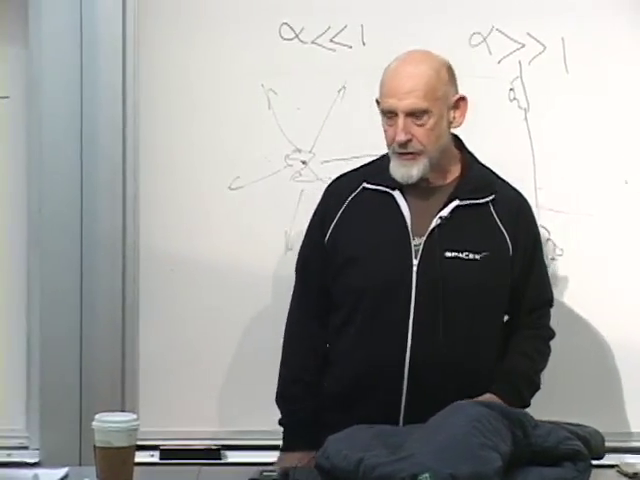
\includegraphics[width=0.72\textwidth]{lecture_01_figure_02.png}
\lectureframe{00:38:22.500}

\vspace{1em}

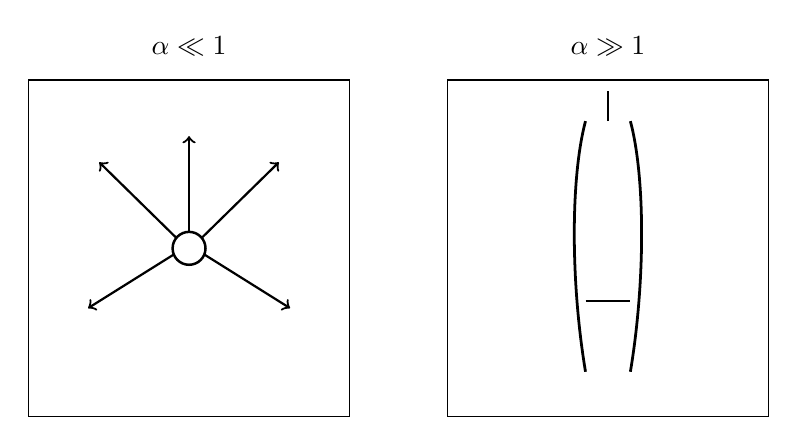
\begin{tikzpicture}[scale=0.95]
\draw (-5.3,-2.4) rectangle (-1.0,2.1);
\draw (0.3,-2.4) rectangle (4.6,2.1);

\node at (-3.15,2.55) {$\alpha \ll 1$};
\node at (2.45,2.55) {$\alpha \gg 1$};

\draw[line width=0.9pt] (-3.15,-0.15) circle (0.22);
\draw[->,line width=0.8pt] (-3.15,0.07) -- (-3.15,1.35);
\draw[->,line width=0.8pt] (-2.98,-0.01) -- (-1.95,1.00);
\draw[->,line width=0.8pt] (-3.32,-0.01) -- (-4.35,1.00);
\draw[->,line width=0.8pt] (-2.95,-0.23) -- (-1.80,-0.95);
\draw[->,line width=0.8pt] (-3.35,-0.23) -- (-4.50,-0.95);

\draw[line width=1.0pt] (2.15,-1.8) .. controls (1.95,-0.6) and (1.95,0.8) .. (2.15,1.55);
\draw[line width=1.0pt] (2.75,-1.8) .. controls (2.95,-0.6) and (2.95,0.8) .. (2.75,1.55);
\draw[line width=0.8pt] (2.15,-0.85) -- (2.75,-0.85);
\draw[line width=0.8pt] (2.45,1.55) -- (2.45,1.95);
\end{tikzpicture}
\caption{討論相互作用能時呈現的QED弱--強耦合比較。圖中分別呈現Susskind所談的兩種情況：弱耦合時稀薄的雲，以及強耦合時增多的雲。}
\end{figure}

雖然前面已經介紹過弱--強耦合的比較，這張圖之所以放在這裡，是因為講座中Susskind在後面這段由提問引出的討論裡，談到相互作用能與增多的結構時，又重新畫出這項對比。

\section{偶數維膜理論與額外維度的湧現}

到目前為止，講座一直在談不同描述間的互換：費米子與玻色子、電子與磁單極子、F弦與D弦。接下來的發展更加出乎意料。Susskind轉而討論另一種弦理論，其中有偶數維的D膜，而非奇數維的D膜。這項區別很重要，因為在這個理論中，沒有D弦可以與F弦互換。理論中有D0膜、D2膜、D4膜，依此類推。

因此，強耦合極限不能只是把一種弦重新標記成另一種弦。按照講座的說法，發生的事情更加奇特：一個額外的空間維度顯現出來。Susskind刻意先用最戲劇化的說法表達---``一個新維度實體化''---，接著立刻改用較謹慎的說法解釋：原本極小的緊緻方向逐漸擴大，直到再也不能忽略。

維度的計數本身就是重點之一，因此他特別停下來說明：
\begin{equation}
\begin{aligned}
10\text{-dimensional string theory} &= 9\text{ space}+1\text{ time},\\
11\text{-dimensional theory} &= 10\text{ space}+1\text{ time}.
\end{aligned}
\end{equation}
講座主張，偶數維膜理論的強耦合極限，實際上是十一維理論。

\editorialnote{偶數維膜理論是IIA型弦理論，其強耦合完備理論是M理論。在標準單位下，湧現的圓周半徑與十一維普朗克長度分別按\(R_{11}=g_s\ell_s\)和\(\ell_{11}=g_s^{1/3}\ell_s\)的關係縮放。這些名稱與公式明確呈現了講座幾何圖像背後的現代對應關係。}

\subsection{花生醬三明治}

為了想像這個緊緻方向，Susskind使用``花生醬三明治''模型：兩片無限薄的麵包，中間則是真實空間。這個模型有一項特別規則：從一側出去，就會從另一側回來。講座以圖像而非形式方式說明這個模型；若用一種常見記號表示，可以寫成
\begin{equation}
y \sim y + 2\pi R.
\end{equation}
如果\(R\)很小，生活在三明治中的觀察者就會把自己的世界視為低維世界。強耦合時的關鍵變化則是
\begin{equation}
g\uparrow
\qquad \Longrightarrow \qquad
R_{\mathrm{compact}}\uparrow.
\end{equation}
Susskind所說「新的空間維度出現」，指的不是空間無中生有，而是原本極小的緊緻方向擴大，在有效理論中變得可見。

\begin{figure}[htbp]
\centering
\resizebox{\linewidth}{!}{%
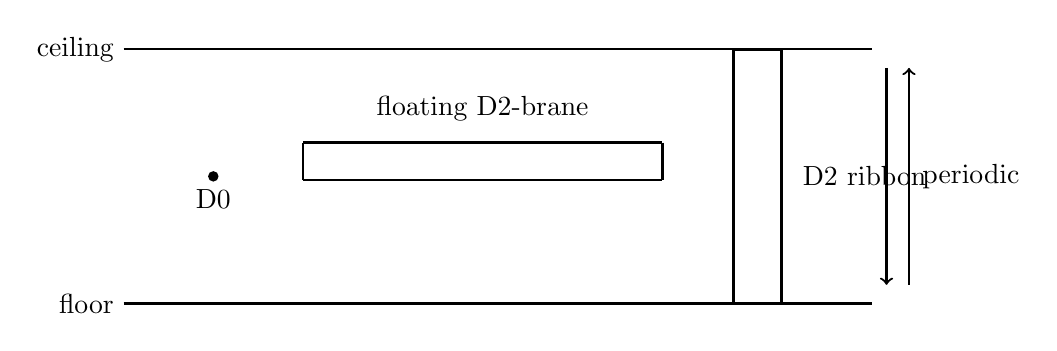
\begin{tikzpicture}[scale=0.95]
\draw[line width=0.9pt] (-5,1.7) -- (5,1.7);
\draw[line width=0.9pt] (-5,-1.7) -- (5,-1.7);

\node[left] at (-5,1.7) {ceiling};
\node[left] at (-5,-1.7) {floor};

\draw[->,line width=0.8pt] (5.2,1.45) -- (5.2,-1.45);
\draw[->,line width=0.8pt] (5.5,-1.45) -- (5.5,1.45);
\node[right] at (5.55,0) {periodic};

\draw[line width=1.0pt] (-2.6,0.45) -- (2.2,0.45);
\draw[line width=1.0pt] (-2.6,-0.05) -- (2.2,-0.05);
\draw[line width=1.0pt] (-2.6,0.45) -- (-2.6,-0.05);
\draw[line width=1.0pt] (2.2,0.45) -- (2.2,-0.05);
\node at (-0.2,0.9) {floating D2-brane};

\draw[line width=1.0pt] (3.15,-1.7) -- (3.8,-1.7);
\draw[line width=1.0pt] (3.15,1.7) -- (3.8,1.7);
\draw[line width=1.0pt] (3.15,-1.7) -- (3.15,1.7);
\draw[line width=1.0pt] (3.8,-1.7) -- (3.8,1.7);
\node[right] at (3.95,0) {D2 ribbon};

\fill (-3.8,0) circle (0.07);
\node[below] at (-3.8,-0.05) {D0};
\end{tikzpicture}
}%
\caption{三明治緊緻化。上下邊界以週期方式識別；一張D2膜像地毯一樣浮在兩者之間，另一張則從地板延伸到天花板。當緊緻方向很小時，後者看起來像一條弦。}
\end{figure}

\subsection{D0膜與D2膜會如何變化？}

講座接著問D0膜和弦會如何變化。兩者的情況並不相同。隨著\(g\)增大，D0膜會愈來愈輕；在高維的詮釋中，它們成為一系列攜帶新顯現方向之動量的粒子。因此，在弱耦合圖像中沉重而複雜的物件，在強耦合圖像中會成為普通的輕激發。

質量關係式呈現了這項對應：
\begin{equation}
M_{D0}(n)=\frac{n}{g_s\ell_s}
=\frac{n}{R_{11}}
=M_{\mathrm{KK}}(n).
\end{equation}
\editorialnote{Susskind稱D0膜為十一維理論中的``引力子''。更精確地說，它們的束縛態是十一維超重力多重態中的Kaluza--Klein動量模態；該多重態的無質量部分包含引力子。這項區分保留了講座所指出的物理對應，也避免把單一粒子說成字面上的等同物。}

D2膜說明了弦的命運。講座著重介紹兩種構型：
\begin{enumerate}
\item 一張D2膜，像花生醬中的地毯一樣浮在地板與天花板之間；
\item 一張D2膜，像緞帶一樣從地板延伸至天花板，沿著可見方向展開。
\end{enumerate}
三明治很薄時，這條緞帶看起來有效上只有一維。低能觀察者稱它為弦。緊緻方向展開後，同一個物件就明確呈現為膜。由於它在垂直方向上延展得更長，包含更多材料，因此變得沉重，也不再像弦。

\paragraph{轉變的邏輯。}
\begin{enumerate}
\item 先從一個極薄的緊緻方向開始，此時從地板延伸到天花板的帶狀結構，從有效描述來看就像一條弦。
\item 增大 \(g\)，緊緻方向便會膨脹。
\item D0-膜變得很輕，並被重新詮釋為高維理論中的 Kaluza--Klein 動量態。
\item 類似弦的 D2帶狀結構則變成明顯延展的膜，並且變得很重。
\end{enumerate}
這是講座從對偶性轉向湧現幾何的關鍵轉折。強耦合不只是把一種物體換成另一種物體；它改變了哪一種幾何描述最有效。

Susskind 停下來談這聽起來有多麼奇特。這些假設的對應關係必須滿足艱深的數學一致性條件；其中有些最初只是物理學家提出的猜想，後來才由數學家證明。他並不是說每一種現實的弦真空都已得到理解，而是說，這套對偶關係網已經通過了異常嚴格的檢驗。

在這個理想化設定中，如果耦合隨位置而變，最有效的幾何描述也可能隨之改變。一個區域可能近似呈現十維描述，其中的弦很輕，D0-膜很重；另一個區域則可能展開為十一維描述，其中包裹膜很重，Kaluza--Klein 模式很輕。這種局部描述方式的改變，正是同一套對偶關係網的一部分。

逐字稿曾短暫把這些關係記作``不等式''。依上下文判斷，原意應是\emph{對偶性}：參數空間兩端之間的對應關係。這項更正很重要，因為講座的結論恰恰是：目前並不知道有一份唯一的基本組分清單。弦、膜、粒子和高維幾何都可以彼此轉化；這表示對偶關係網中可能沒有任何一個成員是絕對基本的，也可能仍有某種更深層的組織方式尚未為人所知。

\section{D3-膜、包裹膜與對偶性的幾何圖像}

休息之後，Susskind 明確地把這個主題描述為一個由相互關聯的理論與觀念構成的``龐大網絡''。接下來的例子並非彼此孤立的新效應，而是連結前面各個例子的橋梁。

\subsection{D3-膜的世界體積}

第一座橋梁以 D3-膜為例。D3-膜有三個空間維度，受限於膜上的觀測者很容易把它當成普通空間。膜可以彎曲、漲落；終止於膜上的弦則可以接合、分裂和散射。對只看得到膜上方向的觀測者而言，每個端點看起來都像粒子，而端點之間的交互作用則像普通的量子場論。

\begin{figure}[htbp]
\centering
\resizebox{\linewidth}{!}{%
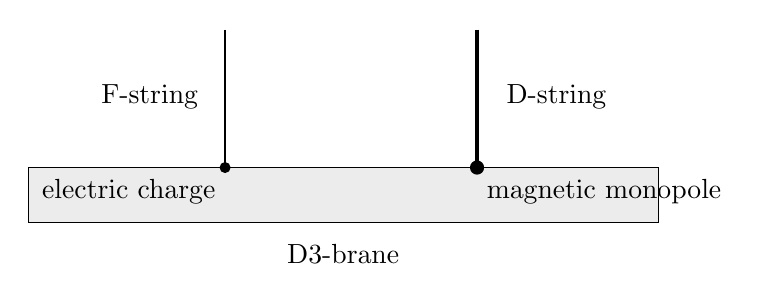
\begin{tikzpicture}[scale=1.0]
\draw[fill=gray!15] (-4,-0.35) rectangle (4,0.35);
\node at (0,-0.75) {D3-brane};

\draw[line width=0.9pt] (-1.5,2.1) -- (-1.5,0.35);
\fill (-1.5,0.35) circle (0.07);
\node[left] at (-1.72,1.25) {F-string};
\node[below left] at (-1.5,0.32) {electric charge};

\draw[line width=1.5pt] (1.7,2.1) -- (1.7,0.35);
\fill (1.7,0.35) circle (0.09);
\node[right] at (1.95,1.25) {D-string};
\node[below right] at (1.7,0.32) {magnetic monopole};
\end{tikzpicture}
}%
\caption{D3-膜世界體積上的詮釋。F 弦端點表現為電荷；D 弦端點表現為磁單極子。}
\end{figure}

這是講座中最令人欣喜的對應之一。終止於 D3-膜上的 F 弦，在世界體積上的觀測者看來是電荷；終止於同一張膜上的 D 弦，則看起來是磁單極子。換句話說，F 弦與 D 弦之間的對偶性，在 D3-膜的世界體積上，成了普通場論中的電--磁對偶性。先前只是一種類比，如今則有了明確的對照關係。

\editorialnote{對一疊 D3-膜而言，低能世界體積描述是四維 \(\mathcal N=4\)超對稱楊---米爾斯理論。這個理論的電--磁對偶性，是 IIB 型弦論 S 對偶在場論中的實現；講座圖示所用的阿貝爾極限則對應單張膜。}

\subsection{兩個緊緻方向與非對稱纏繞}

接著，Susskind 回到高維幾何，將兩個小方向緊緻化，而不是只緊緻化一個。由於十一維無法直接畫在黑板上，他把草圖中未呈現的七個大方向壓縮成一個可見的水平方向，再把兩個緊緻方向明確畫出來。他特意以非對稱的方式畫出緊緻化，因為若要讓有效弦具有不同張力，其中一個緊緻方向就必須比另一個短。

\begin{figure}[htbp]
\centering
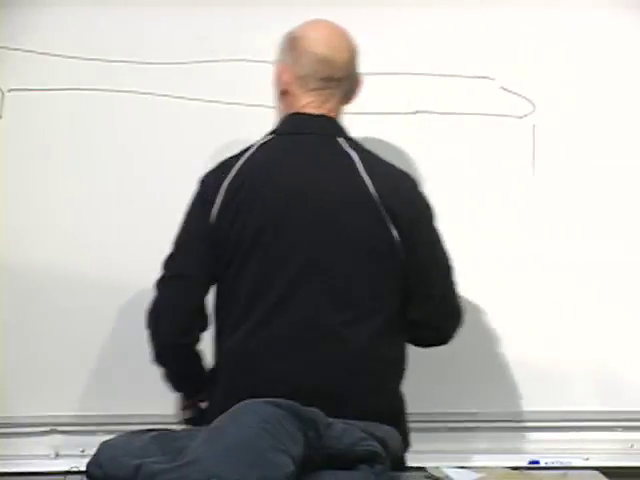
\includegraphics[width=0.78\textwidth]{lecture_01_figure_03.png}
\lectureframe{01:10:25.000}
\caption{兩種包裹膜在黑板上的完整圖示。較短與較長的緊緻迴圈，分別形成右側畫出的類 F 弦與類 D 弦帶狀結構。}
\end{figure}

膜可以纏繞其中一個緊緻方向，從非緊緻方向看去便像一條弦。若 \(R_1\) 和 \(R_2\) 分別是兩個圓的半徑，則有效張力為
\begin{equation}
\begin{aligned}
T_{(1)}&=2\pi R_1 T_{\mathrm{M2}},\\
T_{(2)}&=2\pi R_2 T_{\mathrm{M2}},\\
\frac{T_{(1)}}{T_{(2)}}&=\frac{R_1}{R_2}.
\end{aligned}
\end{equation}
因此，兩個圓的大小不同，有效弦張力也不同。若把沿較短方向纏繞的構型視為輕的 F 弦，把沿較長方向纏繞的構型視為重的 D 弦，便可示意地寫成
\begin{equation}
g_s\sim \frac{R_{\mathrm{short}}}{R_{\mathrm{long}}},
\qquad
\frac{T_{\mathrm{D1}}}{T_{\mathrm{F1}}}\sim \frac{1}{g_s}.
\end{equation}

\begin{classroomqa}
\audiencequestion{這個圖像中的耦合，能否理解為兩個緊緻方向的尺度比？\lecturetimestamp{01:10:13}}
\lecturerresponse{可以。弱--強耦合參數可以幾何化為長寬比。縮短其中一個方向會得到小耦合；交換兩個方向，則會交換輕弦與重弦。}
\end{classroomqa}

\editorialnote{講座暫時以 \(\alpha\) 表示這個比值，沿用先前表示 QED 精細結構常數的符號。為了區分這兩種意義，我們在此改用 \(g_s\)。在完整的 M 理論構造中，IIB 型耦合由緊緻二維環面的複結構編碼；分子究竟是哪一個量，取決於如何標記環面的兩個週期。}

不考慮黑板圖的透視變形，包裹膜的圖像可以概括如下：

\begin{figure}[htbp]
\centering
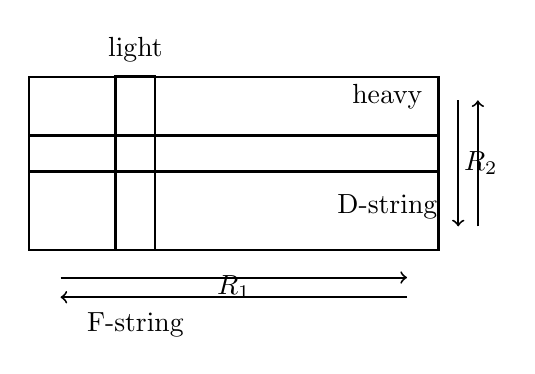
\begin{tikzpicture}[scale=1.0]
\draw[line width=0.9pt] (0,0) rectangle (5.2,2.2);
\node[below] at (2.6,-0.2) {\(R_1\)};
\node[right] at (5.4,1.1) {\(R_2\)};

\draw[->,line width=0.7pt] (5.45,1.9) -- (5.45,0.3);
\draw[->,line width=0.7pt] (5.7,0.3) -- (5.7,1.9);
\draw[->,line width=0.7pt] (0.4,-0.35) -- (4.8,-0.35);
\draw[->,line width=0.7pt] (4.8,-0.6) -- (0.4,-0.6);

\draw[line width=1.0pt] (1.1,0) -- (1.6,0) -- (1.6,2.2) -- (1.1,2.2) -- cycle;
\node at (1.35,2.55) {light};

\draw[line width=1.0pt] (0,1.45) -- (5.2,1.45);
\draw[line width=1.0pt] (0,1.00) -- (5.2,1.00);
\node at (4.55,1.95) {heavy};

\node at (1.35,-0.95) {F-string};
\node at (4.55,0.55) {D-string};
\end{tikzpicture}
\caption{從非緊緻方向看去，兩種包裹膜構型都像弦；但緊緻方向的尺度不同，會使其中一種有效弦比另一種輕。}
\end{figure}

這是前述對偶故事的幾何版本。縮小一個方向、同時拉長另一個方向，會使一種包裹構型變重，另一種變輕，因此 F 弦與 D 弦的角色可以互換。

\begin{classroomqa}
\audiencequestion{如果緊緻方向是週期性的，纏繞物件會不會寬到無限大？\lecturetimestamp{01:10:41}}
\lecturerresponse{不會。緊緻圓的周長有限，即使可以沿圓周不斷繞行，也不會遇到邊界。剖開後圖像的上端與下端代表同一個點，就像一個區間的兩端可以代表圓上的同一點。}
\end{classroomqa}

\begin{figure}[htbp]
\centering
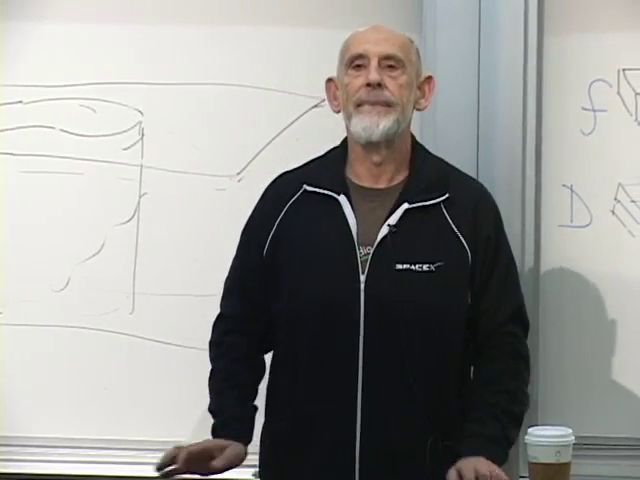
\includegraphics[width=0.78\textwidth]{lecture_01_figure_04.png}
\lectureframe{01:12:25.000}

\vspace{1em}

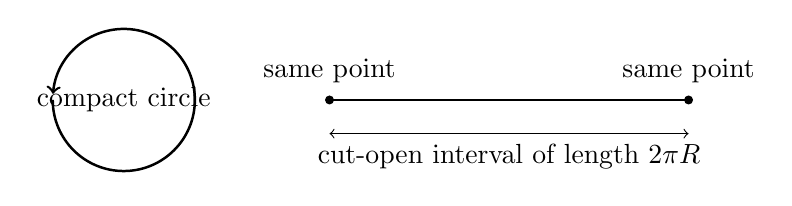
\begin{tikzpicture}[scale=0.95]
\draw[line width=0.9pt,->] (-3.7,0) arc[start angle=180,end angle=535,radius=0.95];
\node at (-2.75,0) {compact circle};
\draw[line width=0.9pt] (0.0,0) -- (4.8,0);
\fill (0.0,0) circle (0.06);
\fill (4.8,0) circle (0.06);
\draw[<->] (0.0,-0.45) -- (4.8,-0.45);
\node at (2.4,-0.75) {cut-open interval of length \(2\pi R\)};
\node[above] at (0.0,0.1) {same point};
\node[above] at (4.8,0.1) {same point};
\end{tikzpicture}
\caption{緊緻圓及其剖開後的黑板表示圖。越過一端會從另一端接回；若在沿圓周移動的同時也沿非緊緻方向前進，描出的路徑則會是螺旋線。}
\end{figure}

\begin{classroomqa}
\audiencequestion{為什麼緊緻路徑是圓，而不是螺旋線？\lecturetimestamp{01:12:23}}
\lecturerresponse{在非緊緻方向的每一個固定位置，緊緻方向都是一個圓。只有當物體沿非緊緻方向前進時又同時繞著圓周移動，才會形成螺旋線。黑板上的區間只是把圓剖開，並將兩端視為同一點。}
\end{classroomqa}

\begin{classroomqa}
\audiencequestion{這種幾何本身能否說明，為什麼近距離探測 D 膜時，它看起來會像由許多 F 弦構成？\lecturetimestamp{01:12:49}}
\lecturerresponse{兩者確實有關聯，但在這個初步圖像中並不明顯；要看出這層關聯，需要更多幾何工具。這張圖是用來整理對偶關係，並非要推導每一種微觀組分描述。}
\end{classroomqa}

\begin{classroomqa}
\audiencequestion{長、短緊緻方向是否可能隨著位置改變或時間演化而互換？\lecturetimestamp{01:13:35}}
\lecturerresponse{在理想化模型中，兩種情況都有可能。壓縮一個週期、同時擴張另一個週期，便會改變哪一種纏繞弦較輕。這也說明了為什麼``基本弦''只是一個名稱：較合適的描述可能因區域或時間而異。}
\end{classroomqa}

\section{理想化、特殊對稱點與景觀}

講座最後一部分從優雅的對偶性例子退一步，探討這些例子能告訴我們什麼，以及不能告訴我們什麼。

首先，Susskind 提醒聽眾，那些能精確掌握的對偶性，是高度理想化的超對稱理論所具有的特徵；在這些理論中，玻色子與費米子的質量完全相同。他以牛頓力學中的圓軌道為例：人們先研究圓軌道，是因為它對稱且容易用數學處理，而不是因為實際的行星運動全都能以完美圓軌道描述。同理，超對稱弦論較容易分析，是因為它們比自然界所呈現的情況更具對稱性。

不過，理想化仍然有助於理解物理。完美的圓軌道並非真實的行星系統，卻能顯示在對稱性較低的軌道中仍然存在的特徵。同樣地，超對稱例子展示了量子力學、引力與微觀結構能夠彼此協調的自洽方式。Susskind 刻意用鮮明的說法指出：那些容易處理的弦論，並非字面意義上描述我們世界的理論；它們的價值在於揭示一些現象，而這些現象很可能也會出現在對稱性較低、較難處理的情況中。

\subsection{能產生多種結果的構造工具}

D 膜只是可用構造工具的一部分。講座也提到通量、軌形與定向軌形。首先選定一種緊緻幾何，再選擇哪些膜與通量佔據其中的週期。即使是簡單的三明治構型，只要放入一個、兩個或三個漂浮的 D2-膜，其低維物理也會改變。增減這些成分，會改變有效粒子、交互作用與參數。

假設依照講座中的示意性計數，一個六維緊緻空間大約有 \(500\) 個週期，而每個週期大約有 \(10\) 種可選的包裹膜、通量或相關結構。那麼構造的數量便會按下式增長：
\begin{equation}
N_{\mathrm{vacua}} \sim 10^{500}.
\end{equation}
講座中的計數方式很簡單：
\begin{equation}
10 \times 10 \times \cdots \times 10 = 10^{500}
\end{equation}
其中有 \(500\) 個因子。DNA 的類比用更熟悉的方式表達了同一點：
\begin{equation}
N_{\mathrm{DNA}}(500)=4^{500}.
\end{equation}
談到 DNA 時，一位聽眾確認，一條鏈上有四種可能：A、C、G 和 T。這項更正強化了原本的論點，並未改變論點。少數局部選擇重複許多次，就會產生數量龐大的整體排列。確切的指數並非重點；Susskind 稱 \(10^{500}\) 是過去的低估，重點在於組合數目急遽增長。

這讓講座一開始的還原論期待徹底翻轉。複雜的粒子物理未必源自複雜的微觀規則；它也可能是因為我們的真空由許多簡單成分組成，並以複雜的方式排列而成，就像複雜生物體可以由四種鹼基構成的序列編碼。

\begin{classroomqa}
\audiencequestion{在把由對偶性聯繫的等價描述視為相同之後，完整資訊是否能從這些可能的真空中，選出一個或少數幾個來描述我們的世界？\lecturetimestamp{01:26:11}}
\lecturerresponse{想必它會選出其中一部分，但許多不同的真空在可達能量範圍內可能看起來極為相似。所引述的景觀估計，即使在把對偶描述視為相同之後，數目仍然很大；而不相關的高能細節可能就像``垃圾 DNA''}一樣。\end{classroomqa}

\subsection{對稱點與一般情況下的複雜性}

景觀中存在一些特別對稱的點。在幾何圖像中，長寬相等的構型
\begin{equation}
R_1=R_2,
\end{equation}
會讓兩種包裹構型同樣簡單。在電--磁類比中，這種情況可示意地表示為
\begin{equation}
m_{\mathrm{monopole}}=m_e.
\end{equation}

\begin{figure}[htbp]
\centering
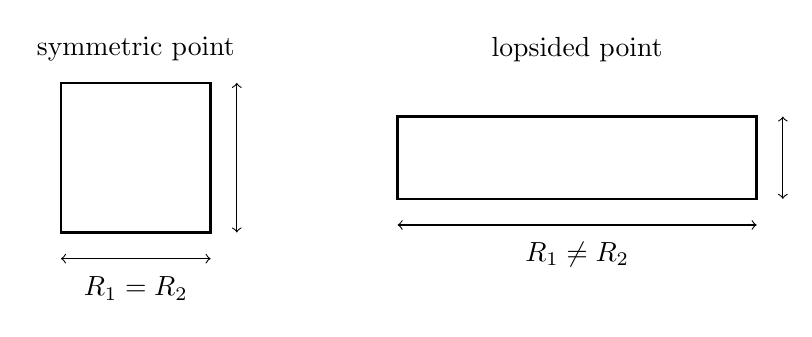
\begin{tikzpicture}[scale=0.95]
\draw[line width=0.9pt] (-4.5,-1.0) rectangle (-2.5,1.0);
\draw[<->] (-4.5,-1.35) -- (-2.5,-1.35);
\draw[<->] (-2.15,-1.0) -- (-2.15,1.0);
\node at (-3.5,1.45) {symmetric point};
\node at (-3.5,-1.75) {$R_1=R_2$};

\draw[line width=0.9pt] (0.0,-0.55) rectangle (4.8,0.55);
\draw[<->] (0.0,-0.9) -- (4.8,-0.9);
\draw[<->] (5.15,-0.55) -- (5.15,0.55);
\node at (2.4,1.45) {lopsided point};
\node at (2.4,-1.3) {$R_1\ne R_2$};
\end{tikzpicture}
\caption{長寬相等的緊緻化對兩種包裹弦一視同仁；長寬不等的緊緻化則使其中一種描述所對應的弦輕得多。}
\end{figure}

\begin{classroomqa}
\audiencequestion{景觀中是否有某些真空，能讓構造簡化許多，因為 F 弦與 D 弦的描述在其中重合？\lecturetimestamp{01:27:21}}
\lecturerresponse{有，確實存在特別對稱的點。我們的世界似乎不在其中：熟悉的帶電粒子與磁單極子的質量並不相等。自然為何位於一個不對稱的點，目前仍然未知。}
\end{classroomqa}

\editorialnote{電子--與磁單極子質量相等，是在適當保護下的自對偶模型所具有的示意性特徵，並非一般非超對稱 QED 的預言。這表達的是講座中關於對稱點的想法，並不是對觀測到的電子所作的主張。}

接著，Susskind 回顧了通訊理論中的一個類比。隨機碼可能極為優良；但最容易描述和解碼的碼往往具有額外的數學結構，過去的表現反而較差。編碼理論後來找到了效率很高的結構化構造，但這個類比仍有啟發性：任何可以用簡短名稱或描述表達的東西，在所有可能性的空間中都只占一個非常特殊、複雜度很低的角落。同樣地，最容易計算的弦真空也可能是非典型的簡單情況。

因此，值得探問的問題或許也會改變。與其要求精確掌握每個微觀細節中的緊緻化方式，不如探問哪些特徵在廣泛的系綜中普遍存在。Susskind 將此視為研究問題，而不是已確立的結論；他也反對以意識形態論證取代計算。

\subsection{宇宙學問題}

\begin{classroomqa}
\audiencequestion{周長極大的緊緻方向，與無限延伸的方向在觀測上有何不同？我們是否知道三個大空間維度是無限的？\lecturetimestamp{01:30:03}}
\lecturerresponse{我們不知道它們是否無限。一個閉合的三維球面可以在保持緊緻的情況下膨脹。對近乎平坦的觀測只能給出曲率半徑的下限；這就像勘測一片近乎平坦的田地，可以推知地球的大小，卻無法證明地球表面是無限的。只有探測到曲率或全域識別關係，才能確定其有限尺度。}
\end{classroomqa}

\begin{classroomqa}
\audiencequestion{如果在理想化模型中，耦合可以隨空間位置而變，那麼現實世界中的這種變化可能如何發生？\lecturetimestamp{01:32:43}}
\lecturerresponse{不是像對稱性例子中那樣不受限制地平滑變化。稍後將討論一種較符合現實的可能性：耦合在有效定律不同的區域之間，透過離散轉變而改變。這種轉變是否會發生，屬於宇宙學問題。}
\end{classroomqa}

\editorialnote{這段回答應理解為講座對通量真空與區域間轉變的預告，而不是一條禁止所有平滑變化標量場的一般定理。觀測對無量綱耦合的變化有很強的限制；而穩定化機制則決定特定模型中是否仍有連續模數可供變化。}

錄音未保留最後一位聽眾的問題。留下來的回答表示，所提到的現象可能發生於某些類型的黑洞，但不會發生在一般史瓦西黑洞的視界處；對自由落下的觀測者而言，該視界在局部看來只是普通的位置。由於無法可靠地還原問題內容，因此不將更具體的主張歸於這段問答。

\section{從磚塊到描述網絡}

認為物理學更深層的內容必定更簡單，這種期待已變得不可靠。在 \(1+1\) 維玻色化中，同一個理論可以用費米子或玻色子來組織，而費米子會以孤子形式重新出現。在量子電動力學中，弱耦合與強耦合會交換電子和磁單極子的描述角色。在弦論中，F 弦與 D 弦重演了同樣的模式；而在偶數維膜理論中，強耦合帶來更進一步的變化：一個緊緻方向膨脹，D0-膜變成 Kaluza--Klein 動量態，有效弦則被重新詮釋為高維幾何中包裹的膜。因此，現代量子場論與弦論並未對``哪些是磚塊、哪些是房屋？''這個問題給出唯一而永久的答案。它們提供的是一個描述網絡，每種描述都在各自的適用範圍內有效；此外還有龐大的可能構造景觀，其一般結果是複雜，而非簡單。
